\section{Parte negativa y positiva}

\begin{definition}[Función truncada]
    Dada una función $f \in M(X, \mathfrak{X})$, para cada $n \geq 1$ definimos la función truncada a $[-n ,n]$ como la $f_n : X \to \R$ dada por
    \begin{align*}
        f_n(x) = \begin{cases}
                     f(x) & \text{si } f(x) \in [-n, n] \\
                     n    & \text{si } f(x) > n         \\
                     -n   & \text{si } f(x) < -n
                 \end{cases}
    \end{align*}
    Que converge puntualmente a $f$.
\end{definition}

Notemos que $f_n$ es medible para todo $n \geq 1$. Pues \begin{align*}
    \{ f_n > \alpha \} = \begin{cases}
                             X                & \text{si } \alpha \leq -n     \\
                             \{ f < \alpha \} & \text{si } \alpha \in [-n, n] \\
                             \varnothing        & \text{si } \alpha \geq n
                         \end{cases}
\end{align*}

Veamos una forma alternativa de probar el teorema de la clase anterior.
Si $f, g \in M(X, \mathfrak{X})$ entonces $f + g: X \to \R \in M(X, \mathfrak{X})$

Para cada $n \geq 1$ consideramos las funciones truncadas $f_n, g_n : X \to \R$.
Tenemos que $f_n + g_n : X \to \R$ es $\mathfrak{X}$-medible. Queremos ver que la convergencia es puntual $\forall x \in X$.

Si $x \in E_1 = \{ f = +\infty \text{, } g = -\infty \}$. Para cada $n \geq 1$,
$f_n(x) = n$ y $g_n(x) = -n$ entonces $(f_n + g_n)(x) = f_n(x) + g_n(x) = 0 \quad (\forall n)$.
Luego $(f_n + g_n)(x) \to 0 = f(x)$ si $x \in E_1$. Para $x \in E_2$ el desarollo es análogo.

Si $x \in (E_1 \cup E_2)^c$ entonces \begin{enumerate}
    \item $f(x)g(x) \in \R$.
    \item $f(x) \in \R$ y $g(x) = +-\infty$.
    \item $f(x) = +-\infty$ y $g(x) \in \R$.
    \item $f(x) = g(x) = +-\infty$.
\end{enumerate}

Luego $(f_n + g_n)(x) \to (f+g)(x) \quad \forall x \in (E_1 \cup E_2)^c$. Pues $f_n(x) \to f(x)$ y $g_n(x) \to g(x)$.

\clearpage

\begin{definition}
    Dada una función $f : X \to \overline{\R}$ definimos la parte positiva $f^{+} : X \to \overline{\R}$ y la parte negativa $f^{-} : X \to \overline{\R}$ como
    \begin{align*}
        f^{+}(x) = \begin{cases}
                       f(x) & \text{si } f(x) \geq 0 \\
                       0    & \text{si } f(x) < 0
                   \end{cases}
    \end{align*}
    \begin{align*}
        f^{-}(x) = \begin{cases}
                       -f(x) & \text{si } f(x) \leq 0 \\
                       0     & \text{si } f(x) > 0
                   \end{cases}
    \end{align*}
\end{definition}

\begin{note}
    $f = f^{+} - f^{-}$ y $|f| = f^{+} + f^{-}$.
\end{note}

\begin{note}
    Si $(X, \mathfrak{X})$ es un espacio medible $f \in M(X, \mathfrak{X}) \iff f^{+} \text{, } f^{-} \in M^{+}(X, \mathfrak{X}) = \{ f \in M(X, \mathfrak{X}) : f \geq 0 \}$
    Notemos que $f^{+} = sup(\{ f, 0 \})$ y $f^{-} = sup(\{ -f, 0 \})$.
    Utilizando el teorema anterior vemos que si $f^{+} \text{, } f^{-} \in M(X, \mathfrak{X})$ entonces $f = f^{+} + (-f^{-}) \in M(X, \mathfrak{X})$.
\end{note}

\begin{note}
    Si $B_f = \{ f = +\infty \}$,
    \[ f^+ = \chi_{B_f^c} \cdot \frac{1}{2} \cdot (f + |f|) \]
    \[ f^- = \chi_{A_f^c} \cdot \frac{1}{2} \cdot (|f| - f) \]
\end{note}

\clearpage

Veamos el siguiente teorema.

Si $f \in M^+(X \text{, } \mathfrak{X})$ entonces $\exists (\phi_n)_{n \geq 1} \in M^+(X \text{, } \mathfrak{X})$ tal que \begin{enumerate}
    \item $\phi_n \leq \phi_{n+1} \quad \forall n \geq 1$.
    \item $f(x) = \lim_{n \to \infty} \phi_n(x) \quad \forall x \in X$.
    \item Para cada $n \geq 1$ se tiene que $\phi_n : X \to \R$ toma una cantidad finita de valores.
\end{enumerate}
\begin{center}
    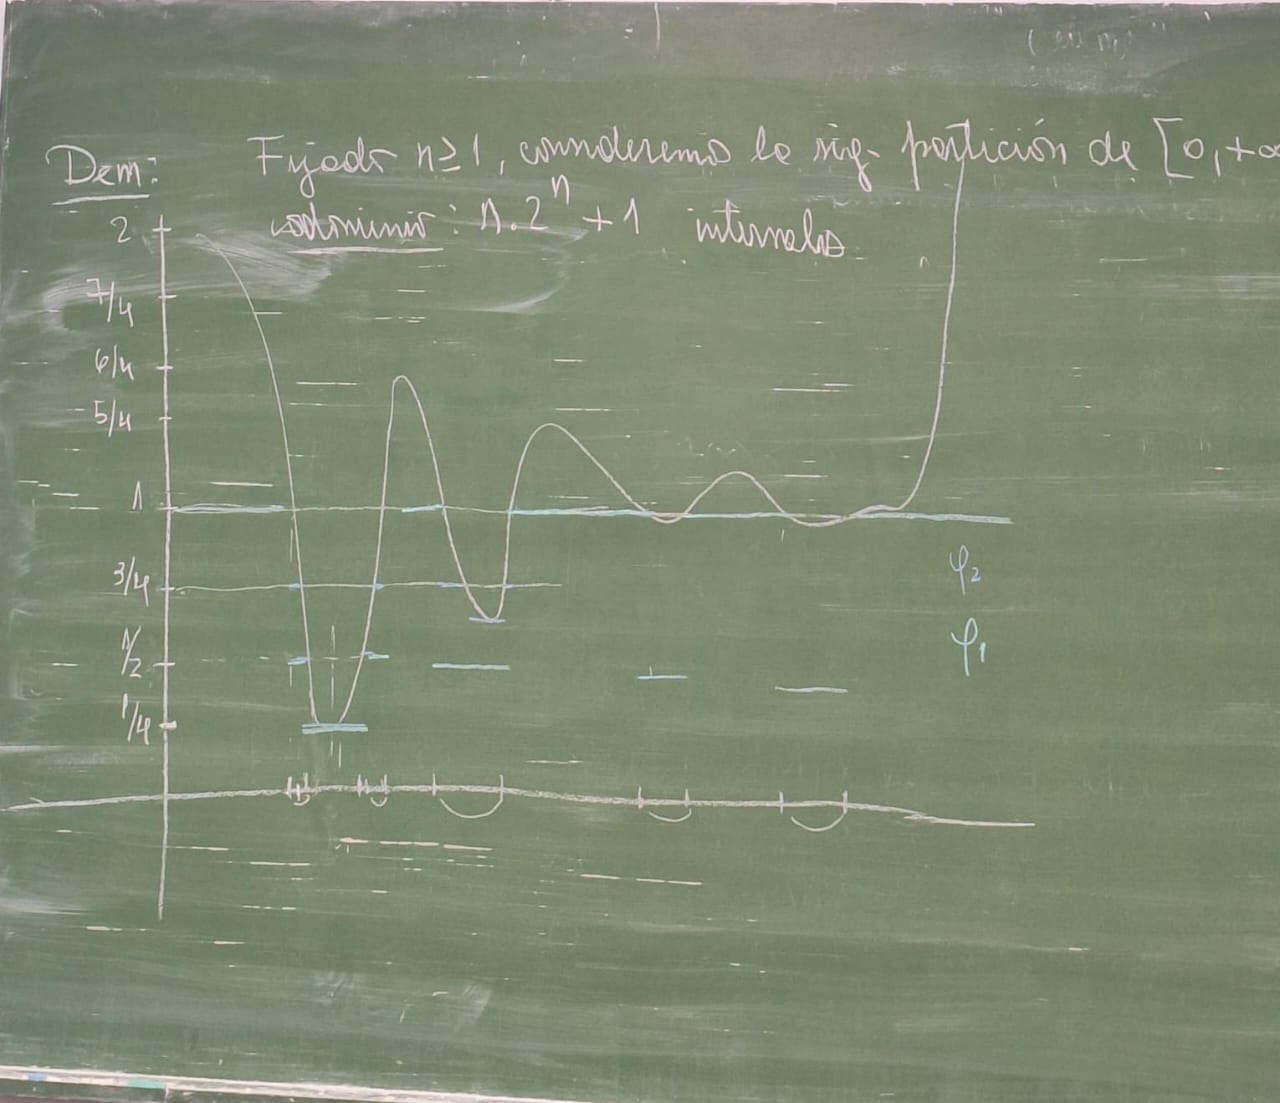
\includegraphics[width=1\textwidth]{Images/clase4.jpeg}
\end{center}
Luego fijado el $n \in \N$ tenemos los intervalos \begin{align*}
    [0, \frac{1}{2}), [\frac{1}{2^n}, \frac{2}{2^n}), \cdots, [\frac{2^{n-1}}{2^n}, \frac{2^n}{2^n}),
    [\frac{2^n}{2^n}, \frac{2^n+1}{2^n}), \cdots, [\frac{n \cdot 2^n - 1}{2^n}, \frac{n \cdot 2^n}{2^n}), [n, +\infty]
\end{align*}
Para cada $k = 0, \cdots, n \cdot 2^n - 1$ definimos el conjunto
\begin{align*}
    E_{k, n} & = f^{-1}([\frac{k}{2^n}, \frac{k+1}{2^n})) \in \mathfrak{X} \\
             & = \{ x \in X : \frac{k}{2^n} \leq f(x) < \frac{k+1}{2^n} \}
\end{align*}
Sea \begin{align*}
    E_{n \cdot 2^n, n} = f^{-1}([n, +\infty]) = \{ x \in X : f(x) \geq n \} \in \mathfrak{X}
\end{align*}

Notemos que $E_{k, n} \in \mathfrak{X} \quad \forall k$, $\bigcup_{k = 0}^{n \cdot 2^n} E_{k, n} = f^{-1}([0, +\infty]) = X$ son disjuntos dos a dos.
Luego definimos $\phi_n(x) = \sum_{k = 0}^{n \cdot 2^n} \frac{k}{2^n} \cdot \chi_{E_{n, k}} = \frac{k}{2^n}$ si $x \in E_{k, n}$, cada $x$ pertenece a un único $E_{k, n}$ por construcción.
Entonces $\phi_n \in M^+(X ,\mathfrak{X})$.

Veamos que $\phi_n \leq \phi_{n+1}$, dado $x \in X$ supongamos que $f(x) < n$ entonces $\exists! k = 0, \cdots, n \cdot 2^n - 1 : x \in E_{k, n}$ (pues en el nivel $n$, son disjuntos).
Queda como ejercicio probar que $E_{k, n} = E_{2k, n+1} \cup E_{2k+1, n+1}$.

Luego
\begin{align*}
    \phi_n(x) = \frac{k}{2^n}
\end{align*}
\begin{align*}\phi_{n+1}(x) = \begin{cases}
                        \frac{2k}{2^{n+1}} = \frac{k}{2^n}                       & \text{si } x \in E_{2k, n+1}   \\
                        \frac{2k+1}{2^{n+1}} = \frac{k}{2^n} + \frac{1}{2^{n+1}} & \text{si } x \in E_{2k+1, n+1}
                    \end{cases}
\end{align*} $\therefore$ $\phi_n(x) \leq \phi_{n+1}(x)$.

Por otro lado si $f(x) > n \to x \in E_{n \cdot 2^n, n}$ entonces $\phi_n(x) = n$.

Como ahora descomponemos $[n, +\infty]$ en $[n, n+1] \cup [n+1, +\infty]$ para $\phi_{n+1}$ lo tenemos como \begin{align*}
    \bigcup_{k = 0}^{2^{n+1}-1} [ \frac{n \cdot 2^{n+1} + k}{2^{n+1}}, \frac{n \cdot 2^{n+1 + k+1}}{2^{n+1}} ) \cup [n+1, +\infty]
\end{align*}
Si $x \in [n+1, +\infty]$ ya está pues $\phi_{n+1}(x) = n+1 \geq n = \phi_n(x)$.

Luego $\exists ! k = 0, \cdots, n \cdot 2^{n+1} : x \in E_{n \cdot 2^{n+1}+k, n+1}$ y en ese caso
$\phi_{n+1}(x) = \frac{n \cdot 2^{n+1} + k}{2^{n+1}} = n + \frac{k}{2^{n+1}} \geq n = \phi_n(x)$.
Por lo tanto $\phi_n \leq \phi_{n+1}$.

Por úlitmo veamos que $f(x) = lim_{n \to +\infty} \phi_n(x) \quad \forall x \in X$.
\begin{enumerate}
    \item $f(x) = +\infty$ luego $\forall n \geq 1 \quad \phi_n(x) = n \to +\infty$.
    \item $f(x) \in [0, +\infty)$. Consideremos $n_0 \in \N : f(x) < n_0$ luego $\forall n \geq n_0 \quad \exists k = 0, \cdots, n \cdot 2^n - 1 : x \in E_{k, n}$.
          Entonces $\phi_n(x) = \frac{k}{2^n} \leq f(x) \leq \frac{k+1}{2^n} \iff 0 \leq f(x) - \phi_n(x) \leq \frac{1}{2^n}$.
\end{enumerate}
$\therefore \phi_n(x) \to f(x)$.

\begin{note}
    Si $f$ está acotada (superiormente) entonces $\phi_n \rightrightarrows f$.
\end{note}

\section{Funciones medibles entre espacios medibles}

\begin{definition}
    Dados espacios medibles $(X, \mathfrak{X})$ y $(Y, \mathfrak{Y})$ una función $f : X \to Y$ es $(\mathfrak{X}, \mathfrak{Y})$-medible si $f^{-1}(E) \in \mathfrak{X} \quad \forall E \in \mathfrak{Y}$.
\end{definition}

\clearpage

\begin{eg}
    Si $(X, \mathfrak{X})$ es un espacio medible:
    \begin{enumerate}
        \item $f: X \to \R$ es $\mathfrak{X}$-medible $\iff f$ es $(\mathfrak{X}, \mathcal{B})$-medible.
        \item $f: X \to \overline{\R}$ es $\mathfrak{X}$-medible $\iff f$ es $(\mathfrak{X}, \overline{\mathcal{B}})$-medible.
        \item $f: X \to \R^n$, sean $f_j : X \to \R$ las componentes de $f$ entonces $f$ es $(\mathfrak{X}, \mathcal{B})$-medible si y sólo si $f_j$ lo es $\forall j$.
    \end{enumerate}
\end{eg}

\begin{prop}
    Dados un espacio medible $(X, \mathfrak{X})$ y un conjunto $Y$, sea $f: X \to Y$ una función.
    Si $\mathcal{A} \subseteq P(Y) : f^{-1}(A) \in \mathfrak{X} \quad \forall A \in \mathcal{A}$ entonces $f$ es $(\mathfrak{X}, \sigma(\mathcal{A}))$-medible.

    \begin{proof}
        Sea $Z = \{ E \subseteq Y : f^{-1}(E) \in \mathfrak{X} \} \supseteq \mathcal{A}$. Es fácil ver que $Z$ es $\sigma$-álgebra entonces $\sigma(\mathcal{A}) \subseteq Z$.
        Es decir que $f^{-1}(E) \in \mathfrak{X} \quad \forall E \in \sigma(\mathcal{A})$. Luego $f$ es $(\mathfrak{X}, \sigma(\mathcal{A}))$-medible.
    \end{proof}
\end{prop}

\begin{prop}
    Sea $(X, \mathfrak{X})$, $(Y, \mathfrak{Y})$, $(Z, \mathfrak{Z})$ espacios medibles y $f: X \to Y$ y $g: Y \to Z$ funciones $(\mathfrak{X}, \mathfrak{Y})$-medible y $(\mathfrak{Y}, \mathfrak{Z})$-medible respectivamente.
    Entonces $g \circ f : X \to Z$ es $(\mathfrak{X}, \mathfrak{Z})$-medible.
    \begin{proof}
        Fijado $E \in \mathfrak{Z}$ tenemos que $(g \circ f)^{-1}(E) = f^{-1}(g^{-1}(E)) \in \mathfrak{X}$ pues $f$ y $g$ son medibles.
    \end{proof}
\end{prop}